
\begin{algorithm}[!th]
\caption{EUCBV}
\label{alg:eucbv}
\begin{algorithmic}
\State {\bf Input:} Time horizon $T$, exploration parameters $\rho$ and $\psi$.
\State {\bf Initialization:} Set $m:=0$, $B_{0}:=\mathcal{A}$, $\epsilon_{0}:=1$, $M=\big \lfloor \frac{1}{2}\log_{2} \frac{T}{e}\big\rfloor$, $n_{0}=\big\lceil\frac{\log{(\psi T\epsilon_{0}^{2})}}{2\epsilon_{0}}\big\rceil$ and  $N_{0}=Kn_{0}$.
\State Pull each arm once
\For{$t=K+1,..,T$}	
\State Pull arm $i\in \argmax_{j\in B_{m}}\bigg\lbrace \hat{r}_{j} + \sqrt{\frac{\rho(\hat{v}_{j}+2)\log{(\psi T\epsilon_{m})}}{4 z_{j}}} \bigg\rbrace$, where $z_j$ is the number of times arm $j$ has been pulled.
%\State $t:=t+1$
\ArmElim
\State For each arm $i \in B_{m}$, remove arm $i$ from $B_{m}$ if,
\begin{align*}
%%%%%%%%%%%%%%%%%%%%%%%
%& \hat{r}_{i} + \sqrt{\frac{\rho\hat{v}_{i}\log{(\psi T\epsilon_{m})}}{4 z_{i}} + \frac{\rho\log{(\psi T\epsilon_{m})}}{4 z_{i}}} < \max_{{j}\in B_{m}}\bigg\lbrace\hat{r}_{j} -\sqrt{\frac{\rho\hat{v}_{j}\log{(\psi T\epsilon_{m})}}{4 z_{j}} + \frac{\rho\log{(\psi T\epsilon_{m})}}{4 z_{j}}} \bigg\rbrace
%%%%%%%%%%%%%%%%%%%%%%%
 \hat{r}_{i} + & \sqrt{\frac{\rho(\hat{v}_{i}+2)\log{(\psi T\epsilon_{m})}}{4 z_{i}}}  
  < \max_{{j}\in B_{m}}\bigg\lbrace\hat{r}_{j} -\sqrt{\frac{\rho(\hat{v}_{j}+2)\log{(\psi T\epsilon_{m})}}{4 z_{j}}} \bigg\rbrace
\end{align*}
\EndArmElim

\If{$t\geq N_{m}$ and $m\leq M$}
\ResParam
\State $\epsilon_{m+1}:=\frac{\epsilon_{m}}{2}$\vspace{0.5ex}
\State $B_{m+1}:=B_{m}$
\State $n_{m+1}:=\bigg\lceil\frac{\log{(\psi T\epsilon_{m+1}^{2})}}{2\epsilon_{m+1}}\bigg\rceil$
\State $N_{m+1}:=t+|B_{m+1}| n_{m+1}$
\State $m:=m+1$
\EndResParam
\EndIf
\State Stop if $|B_{m}|=1$ and pull ${i}\in B_{m}$ till $T$ is reached.
\EndFor
\end{algorithmic}
%\vspace*{-0.42em}
\end{algorithm}
%\vspace*{-0.42em}

\textbf{The algorithm:} Earlier round-based arm elimination algorithms like Median Elimination \citep{even2006action} and UCB-Improved mainly suffered from two basic problems: \\
\begin{inparaenum}[\bfseries(i)]
\item \textit{Initial exploration:} Both of these algorithms pull each arm equal number of times in each round, and hence waste a significant number of pulls in initial explorations. \\
\item \textit{Conservative arm-elimination:} In UCB-Improved, arms are eliminated conservatively, i.e, only after $\epsilon_{m}<\frac{\Delta_{i}}{2}$, 
% the sub-optimal arm $i$ is discarded with high probability. 
where the quantity $\epsilon_{m}$ is initialized to $1$ and halved after every round. In the worst case scenario when $K$ is large, and the gaps are uniform  ($r_{1}=r_{2}=\cdots=r_{K-1}<r^{*}$) and small this results in very high regret.\\
\end{inparaenum}
%For any round $m$ UCB-Improved pulls all arms $n_{m}=\left\lceil \frac{ 2\log(T\epsilon_{m})}{\epsilon_{m}} \right\rceil$ number of times. The quantity $\epsilon_{m}$ is initialized to $1$ and halved after every round.
\\
	The EUCBV algorithm, which is mainly based on the arm elimination technique of the UCB-Improved algorithm,  remedies these by employing exploration regulatory factor $\psi$ and arm elimination parameter $\rho$ for aggressive elimination of sub-optimal arms. Along with these, similar to CCB \citep{liu2016modification} algorithm, EUCBV uses optimistic greedy sampling whereby at every timestep it only pulls the arm with the highest upper confidence bound rather than pulling all the arms equal number of times in each round. Also, unlike the UCB-Improved, UCB1, MOSS and OCUCB algorithms (which are based on mean estimation) EUCBV employs mean and variance estimates (as in \citet{audibert2009exploration}) for arm elimination. Further, we allow for arm-elimination at every time-step, which is in contrast to the earlier work (e.g., \citet{auer2010ucb}; \citet{even2006action}) where the arm elimination takes place only at the end of the respective exploration rounds. An illustrative flowchart depicting the main steps is shown in Figure \ref{fig:eucbv}.
	
\begin{figure}[!th]
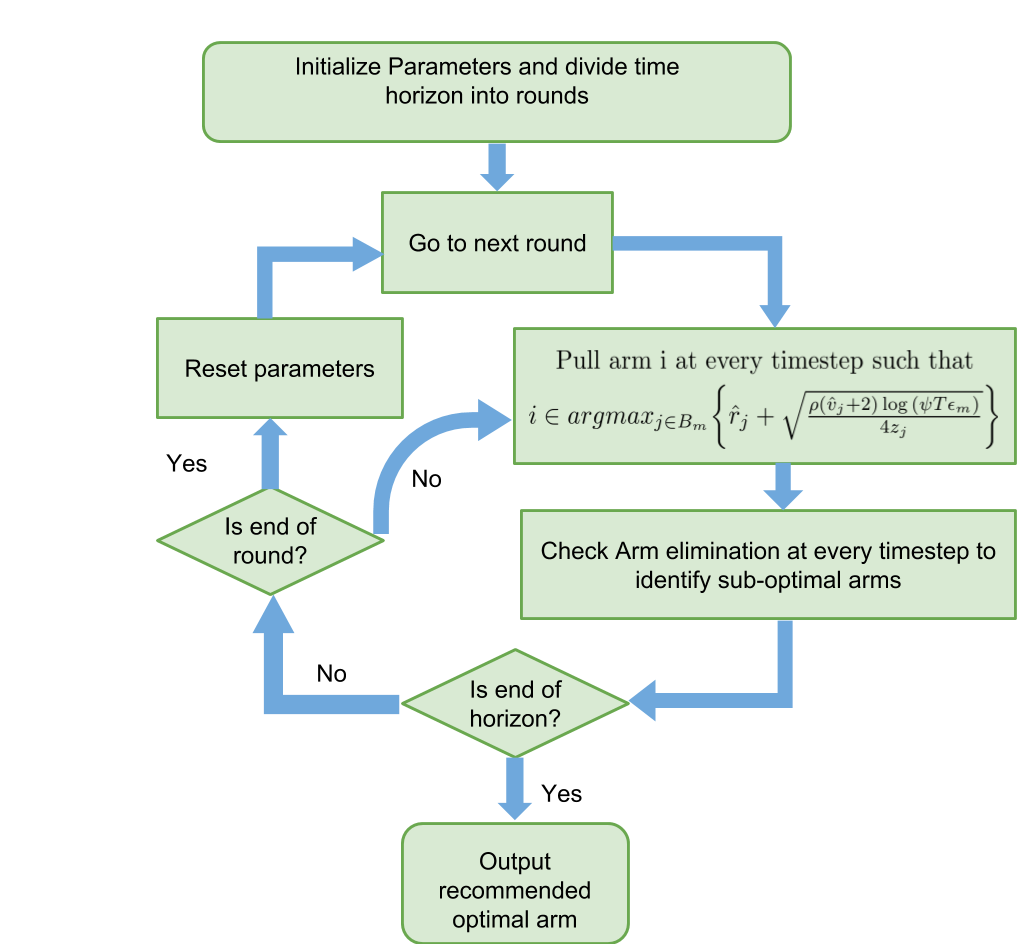
\includegraphics[scale=0.41]{Chapter3/img/EUCBV_flow.png}
\caption{Flowchart of EUCBV algorithm}
\label{fig:eucbv}
\end{figure}




